%%%%%%%%%%%%%%%%%%%%%%%%%%%%%%%%%%%

\chapter{Pebble Interaction Analysis: Theory} \label{sec:analysis-theory}


This chapter will walk through the analysis first performed by Heinrich Hertz in 1880 of idealized interacting spherical objects to represent our ceramic pebbles. We will begin with mechanical interactions of purely elastic spheres and then use the results to develop a theory for conductive heat transfer between the pebbles. Finally, Hertz's theory will also be used to analyze pebble interaction with flat plattens in our test stand used to measure crush force. A relationship is developed allowing us to translate from experimental results to pebble bed ensembles.

%%%%%%%%%%%%%%%%%%%%%%%%%%%%%%%%%%%

% Included sections
\section{Hertz theory for normal contact of spheres}\label{sec:hertz-contact}
[DRAW SOME COORDINATE DIAGRAMS TO SHOW HOW Z R AND X-Y WHATEVER ARE ACTUALLY RELATED AND CAN BE VISUALIZED]
We consider two non-conforming solids approaching and then contacting under load. We only wish to analyze the contact of spheres (of differeng radii), so we are able define the surface curvature of the two contacting bodies as

\begin{align}
z_1 &= \frac{1}{2R_1}r^2 \\
z_2 &= \frac{1}{2R_2}r^2
\end{align}

respectively. The radius, laying in the $x-y$ plane is related to cartesian coordinates as $r^2 = x^2 + y^2$. Before the surfaces are in contact, each point on the two surfaces are separated by a distance $h(r)$,

\begin{align}\label{eq:separationh}
h &= z_1 - z_2 \nonumber \\
h & = \left(\frac{1}{R_1} + \frac{1}{R_2}\right)\frac{r^2}{2} 
\end{align}

We define the relative radius of curvature as

\begin{equation}\label{eq:relativeRadius}
\frac{1}{R^*} = \frac{1}{R_1} + \frac{1}{R_2}
\end{equation}

and then the separation is simply $h = (1/2R^*)r^2$.

\begin{figure}[ht!]
	\begin{center}
	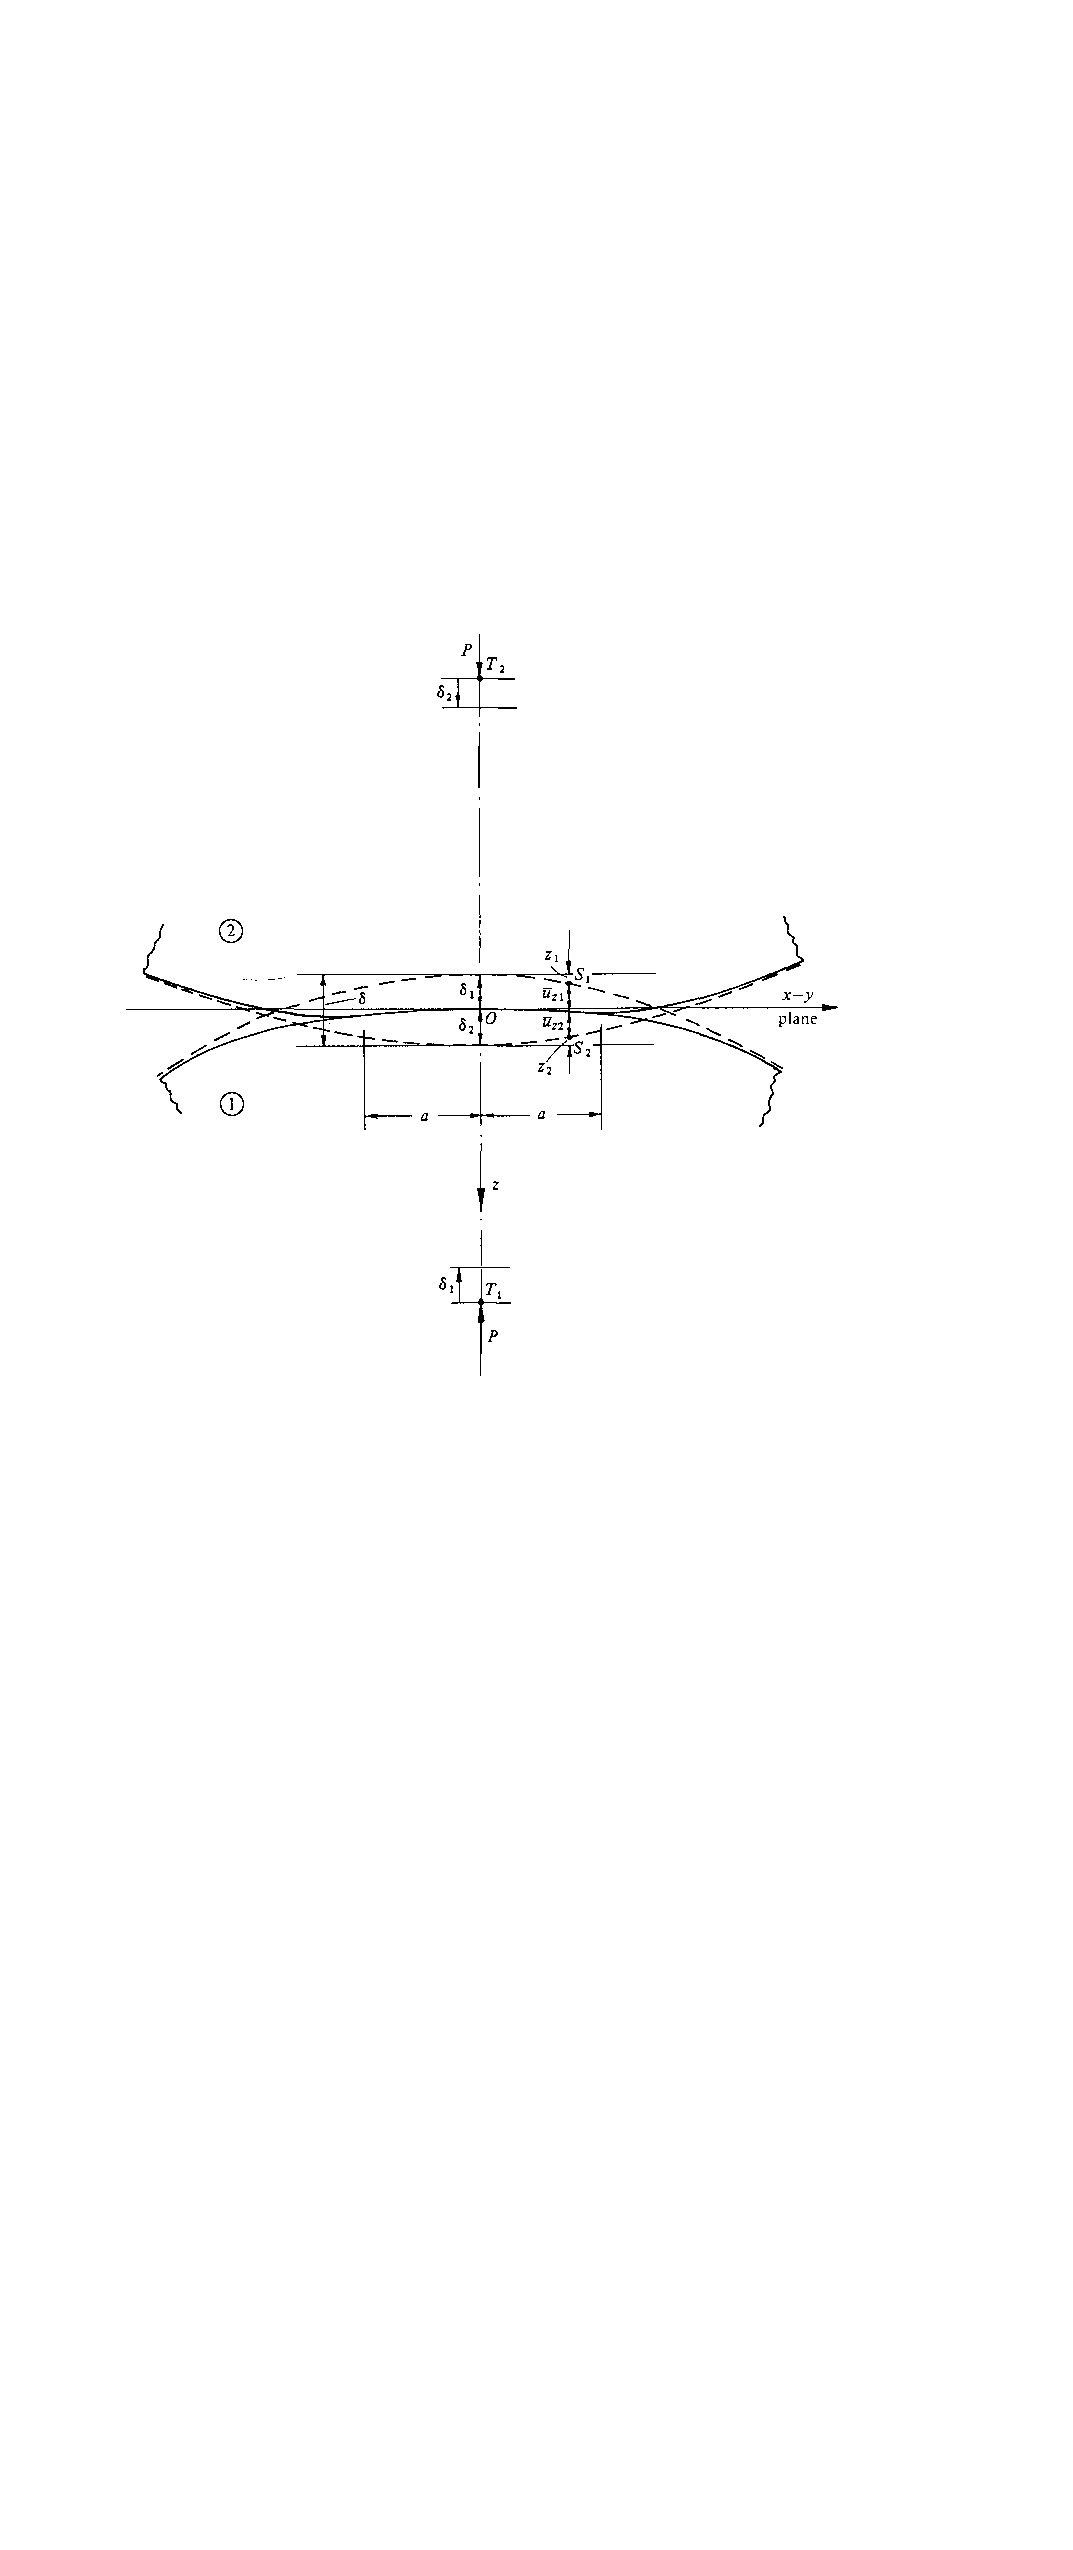
\includegraphics[width=0.95\textwidth]{chapters/figures/hertzGeometry}
	\caption{default}
	\label{fig:hertzgeometry}
	\end{center}
\end{figure}

We allow the two surfaces to approach, and then, under an external load $F$, contact. The cross-section of these bodies after contact are shown in Fig.~\ref{fig:hertzgeometry}. If we first imagine that the two surfaces do not interact and their surfaces pass through each other unimpeded, their surfaces would be overalapped to a distance $\delta$. In such a case, we examine two points deep within the bodies, along the axis of contact, calling them $T_{1}$ and $T_2$. These points will have moved $\delta_1$ and $\delta_2$, respectively. The total overlap is obviously related to these displacements by $\delta = \delta_1 + \delta_2$. 

However, under actual contact, the two surfaces are going to deform as the load $F$ presses them into contact. So now we consider two points on the surfaces, such as $S_1$ and $S_2$. Before contact, these two points are initially are separated by a distance $h$ (from Eq.~\ref{eq:separationh}), then displace by $\bar{u}_{z1}$ and $\bar{u}_{z2}$ due to contact pressure. 

If the points $S_1$ and $S_2$ are inside of the contact region under load, these distances are related by

\begin{equation}
	\bar{u}_{z1} + \bar{u}_{z2} + h = \delta
\end{equation}

Then using Eq.~\ref{eq:separationh}, we have an expression for the elastic displacements:

\begin{equation}\label{eq:hertzdisplacements}
	\bar{u}_{z1} + \bar{u}_{z2} = \delta - \frac{1}{2R^*} \, r^2
\end{equation}

Alternatively, if after deformation the points $S_1$ and $S_2$ are outside of the contact region, this is simply

\begin{equation}\label{eq:hertz-disp-2}
	\bar{u}_{z1} + \bar{u}_{z2} > \delta - \frac{1}{2R^*} \, r^2
\end{equation}

It now is necessary to find a pressure distribution that satisfies these boundary conditions of displacement. Heinrich Hertz first formulated the expressions of Eqs.~\ref{eq:hertzdisplacements,eq:hertz-disp-2} in 1882. The power of his solution is borne out by the continuous use of his theory since that time. Hertz simplified the problem by regarding each body as an elastic half-space upon which the load is applied over a small, elliptical region (the contact area). This simplification allows for treatment of the highly concentrated stresses near the region of contact without consideration of either the general response of stresses in the bulk of the body or the manner in which they are supporting the load. This assumption is justifiable if the dimensions of each body as well as the relative radii of curvature are very large compared to the contact area. These assumptions are sufficient to proceed with the analysis, but the curious are pointed to an excellent discussion and background of Hertz's theory as given in KE Johnson's textbook~\cite{Johnson1985}.

For solids of revolution, a distribution of pressure to satisfy the displacements of Eq.~\ref{eq:hertzdisplacements,eq:hertz-disp-2} is proposed by Hertz as

\begin{equation}
	p = p_0 \left[1-\left(\frac{r}{a}\right)^2\right]^{1/2}
\end{equation}

where $a$ is the radius of the contact area.

The total load, $F$ is found from the pressure distribution as

\begin{align}\label{eq:hertzforcewithpressure}
	F &= \int_0^a \! p(r) 2\pi r\, \mathrm{d}r\\
	F & = \frac{2}{3} p_0 \pi a^2
\end{align}

From the distributed load over the circular region, stresses and deflections are found from superposition of point loads. The pressure is integrated (see Ref.~\cite{Johnson1985}) to find the normal displacement for either solid body as

\begin{equation}
	\bar{u}_z = \frac{1-\nu^2}{E}\frac{\pi p_0}{4a}\left(2a^2 - r^2\right)
\end{equation}

This is applied to both bodies and plugged into Eq.~\ref{eq:hertzdisplacements} to yield

\begin{equation}\label{eq:pressindisplacement}
	\frac{\pi p_0}{4aE^*}\left(2a^2 - r^2\right) = \delta - \left(\frac{1}{2R^*}\right)\, r^2
\end{equation}

where we have introduced the now-common term of pair Young's modulus,

\begin{equation}
	\frac{1}{E^*} = \frac{1-\nu_1^2}{E_1} + \frac{1-\nu_2^2}{E_2}
\end{equation}

for simplification.

With the solution of Eq.~\ref{eq:pressindisplacement}, if we consider $r = a$ and $\delta(a) = 0$, we find the radius of the contact circle is

\begin{equation}
	a = \frac{\pi p_0 R^*}{2E^*}
\end{equation}

and when $r= 0$, we find the overlap as

\begin{equation}
	\delta = \frac{\pi a p_0}{2E^*}
\end{equation}

and alternatively we find the pressure as a function of overlap

\begin{equation}
	p_0 = \frac{2E^*\delta}{\pi a}
\end{equation}

The radius, overlap, and pressure relations are inserted into Eq.~\ref{eq:hertzforcewithpressure} to find the force (from now on referred to as the Hertz force) as a function of overlap, relative radius, and pair Young's modulus,

\begin{equation}\label{eq:hertz-force}
	F = \frac{4}{3}E^* \sqrt{R^*} \, \delta^{3/2}
\end{equation}

Equation~\ref{eq:hertz-force} defines the normal contact forces between any two contacting, elastic spheres. This extremely important result acts as the basis of all discrete element method codes since the concept was first introduced for granular materials by Cundall \& Strack in 1979\cite{Cundall1979}. To differentiate the force from other terms to be derived later, we specificy it as the normal force between sphere $i$ and sphere $j$ as

\begin{equation}\label{eq:hertz-normal-force}
	F_{n,ij} = \frac{4}{3}E_{ij}^* \sqrt{R_{ij}^*} \, \delta_{ij}^{3/2}
\end{equation}







\section{Hertz-Mindlin}\label{sec:hertz-mindlin-theory}
\section{Heat transfer between contacting spheres}

A complete picture of heat transfer of contacting spheres would include internal conduction in the solid material, conduction between contacts, convection to an interstitial gas (as well as partitioning energy carried downstream and energy redeposited locally), and radiation between neighboring solids (on both local and semi-local scales). The first natural step is to focus simply on internal and inter-particle conduction.

[Go back through Batchelor and O'Brien~\cite{Batchelor1977} paper]

\begin{align}
\frac{ k_s }{ k_f } \frac{a}{R^*} = \lambda
\end{align}

Similar to the lumped capacitance assumptions, if $\lambda \gg 1$, the solid is approximately is isothermal. The second group on the left-hand side of this condition we remember from the assumptions of Hertz theory, where we require $\frac{a}{R^*} \ll 1^*$. Therefore to satisfy the condition of $\lambda \gg 1$, we require very large conductivity ratios of solid to fluid, $\frac{k_s}{k_f} \gg 1$. Alternatively this is satisfied by definition if the solids exist in vacuum.

Assuming that we satisfy the condition of isothermal solids, we address the conduction between solids in their small regions of contact.

[more details]

Handling the heat transfer between contacting particles has been investigated extensively by researchers in a number of fields\cite{Zhou2009,Zhang2011,Wu2011,Vargas2001,Li2000,Chaudhuri2006}. The amount of energy per time that can be transported per difference in temperature between pebble $i$ and $j$ as a conductance $h_{ij}$. Defined as
\begin{align}\label{conductance}
\frac{h_{ij}}{k^*}= 2\left[\frac{3F_nR^*}{4E^*}\right]^{1/3}
\end{align}
$k^*= 2k_ik_j/(k_i+k_j)$ is the effective solid conductivity of the two particles, and $F_n$ is the magnitude of the normal force between particles $i$ and $j$ as calculated by Eq.~\ref{eq:hertzForce}. Therefore, if we consider particles at temperatures $T_i$ and $T_j$ in contact, they will transfer heat at a rate of
\begin{align}
Q_{ij} = h_{ij}(T_i - T_j)
\end{align} 
The temperature of particle $i$, for example, is found from the first law of thermodynamics
\begin{align}\label{thermoFirstLaw}
\rho_iV_iC_i\frac{\mathrm{d}T_i}{\mathrm{d}t} = Q_{s,i} + Q_{ij}
\end{align}
where $\rho$, $V$, and $C$ are the density, volume, and the specific heat of the solid, respectively. The energy equation also allows for source heating of the solid with term $Q_{s}$.

\section{Linking interactions with strain energy}\label{theoryStrainEnergy}
Hertz theory is applicable to any two contacting elastic objects. In practice, we cannot probe the contacts of small particles and rely on experiments where we press pebbles between flat platens. Here we will develop a theory for connecting the results of the experiments with the interaction of two spherical objects.

To relate the situation in the lab to two particles, we first integrate the Hertzian force along the overlap to find the strain energy, $W_\epsilon$, of that contact. 
\begin{align}
W_\epsilon & = \int_0^{\delta_c}\!F_n(\delta')\,\mathrm{d}\delta'
\end{align}
where the upper limit of the integration is the critical overlap $\delta_c$ (the meaning of this value will be explained in detail later). With the force defined from Eq.~\ref{eq:hertzForce}, this is straightforward to integrate.
\begin{align}
W_\epsilon& = \int_0^{\delta_c}\!  \frac{4}{3}E^*\sqrt{R^*}\,\delta'^{3/2} \,\mathrm{d}\delta' \\
%W_\epsilon & = \frac{4}{3}E^*\sqrt{R^*} \left[\frac{2}{5}\,{\delta_c}^{5/2}\right] \\
W_\epsilon & = \frac{8}{15}E^*\sqrt{R^*}\, {\delta_c}^{5/2}
\end{align}

We will call the strain energy of the pebble compressed between platens as the lab strain energy, $W_{\epsilon,L}$. The strain energy of two particles in contact will be $W_{\epsilon,B}$. The assumption we make is that, if each interaction is integrated to the proper critical overlap, the strain energies will be equal at that point.
\begin{align}
W_{\epsilon,L} & = W_{\epsilon,B} = \frac{8}{15}E_B^*\sqrt{R_B^*}\, {\delta_{c,B}}^{5/2}
\end{align}

We solve for the interacting particle overlap as a function of the lab strain energy as
\begin{align}
 \delta_{c,B} = \left[\frac{15W_{\epsilon,L}}{8E_B^*\sqrt{R_B^*}}\right]^{2/5}
\end{align}

This overlap can be reinserted to Eq.~\ref{eq:hertzForce} to find the critical force of the interacting particles as a function of the critical strain energy of the lab. Doing this, we find:
\begin{align}\label{eq:peb_hertz}
F_{c,B} = C{E_B^*}^{2/5}{R_B^*}^{1/5}W_{\epsilon,L}^{3/5}
\end{align}
where $C = \frac{4}{3}\left(\frac{15}{8}\right)^{3/5}$.

In this analysis we have referred to a `lab' and `particle' for the two situations. In fact, the result is more general and can be used to relate any two scenarios. The only requirement is that both conditions adhere to the assumptions of Hertz theory. The ramifications of this relationship will be explored in more detail in \S~\ref{analysisExp}.
